\documentclass{beamer}

\usepackage[T1,T2A]{fontenc}
\usepackage[utf8]{inputenc}
\usepackage[russian, english]{babel}

\usepackage{amsmath, amsfonts, amsthm, amscd}
%\usepackage{graphics}
\usepackage{graphicx}
\usepackage[matrix,arrow,curve]{xy}
%\usepackage{multicol}

%----------------------------------------------------

\newtheorem{problemR}{Проблема}
\newtheorem{aim}{Цель}


\newtheorem{construction}{Construction}
\newtheorem{problems}{Problems}
\newtheorem{conjecture}{Conjecture}
\newtheorem{question}{Question}

\mode<presentation>
\usetheme{Madrid}

\title{}
\date{2023}
\author{Бонич Дмитрий}


\begin{document}

\begin{frame}
\begin{center}


{\large \scshape

\bigskip

\bigskip

3d-Renderer с нуля

\bigskip
\bigskip
\bigskip
\bigskip
\bigskip
\bigskip
}

Тип проекта: Программный\\
\bigskip
Выполнил: Бонич Дмитрий, БПМИ 213\\
\bigskip
Научный руководитель: Трушин Дмитрий Витальевич, ФКН ВШЭ 

\end{center}
\end{frame}

\begin{frame}{3D рендеринг}
    3D рендеринг -- процесс выдающий 
    двумерное изображение по некоторому описанию трехмерного объекта.
% TODO: Добавить скриншот: wireframe -> model 
\end{frame}

\begin{frame}

\frametitle{Цель работы и задачи}

Цель: Написать программу способную осуществлять 3D-рендеринг.

\bigskip

Задачи:
\begin{itemize}
    \item Отрисовка 3d-объектов
    \item Загрузка моделей из .obj формата
    \item Освещение
\end{itemize}

\end{frame}

\begin{frame}{Треугольники}
Любой 3d-объект будем аппроксимировать треугольниками.

\begin{center}
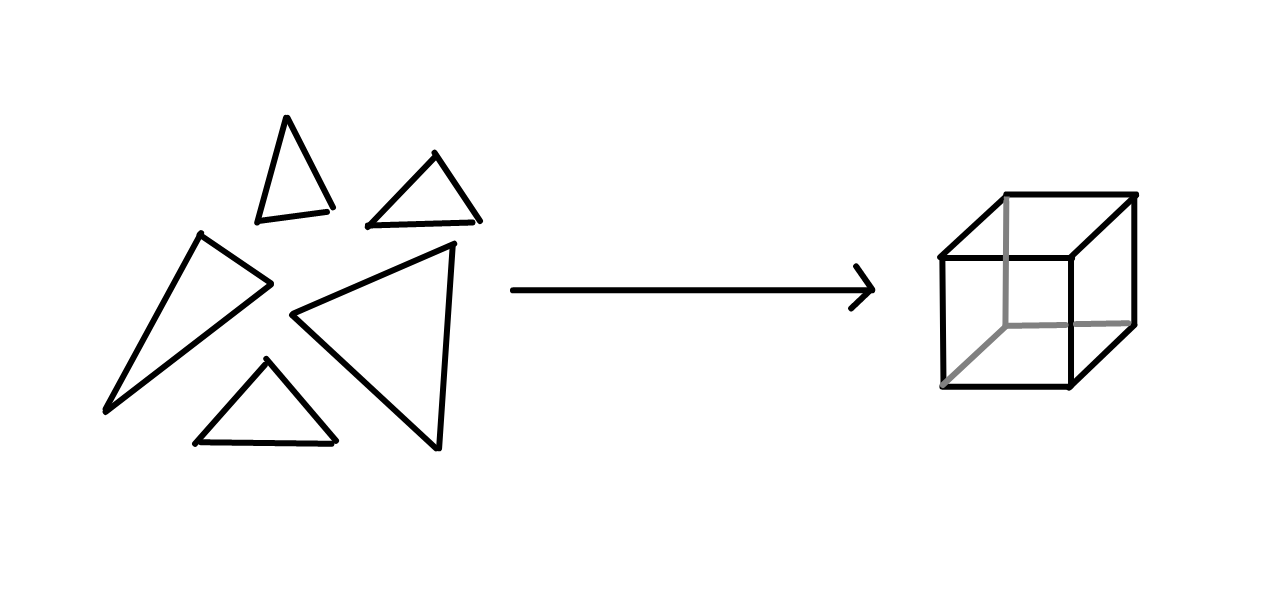
\includegraphics[width=0.6 \linewidth]{triangles.png}
\end{center}

Значит теперь мы хотим научиться рендерить 1 треугольник.

\end{frame}

\begin{frame}{Пайплайн}
\begin{center}
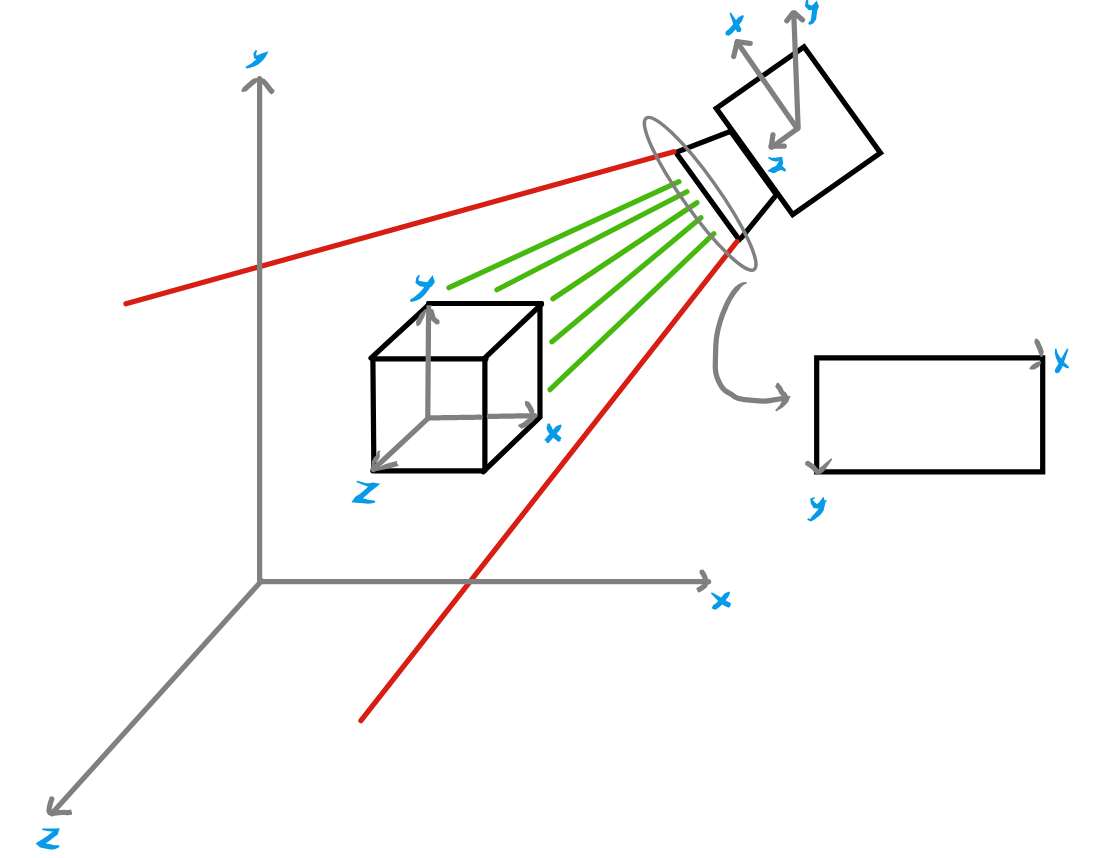
\includegraphics[width=0.86 \linewidth]{coord_systems.png}
\end{center}
\end{frame}

\begin{frame}{Local space}
    Local space -- персональное для каждого объекта пространство в котором нам изначально приходят 
    координаты объекта(например из .obj файла). 
\begin{center}
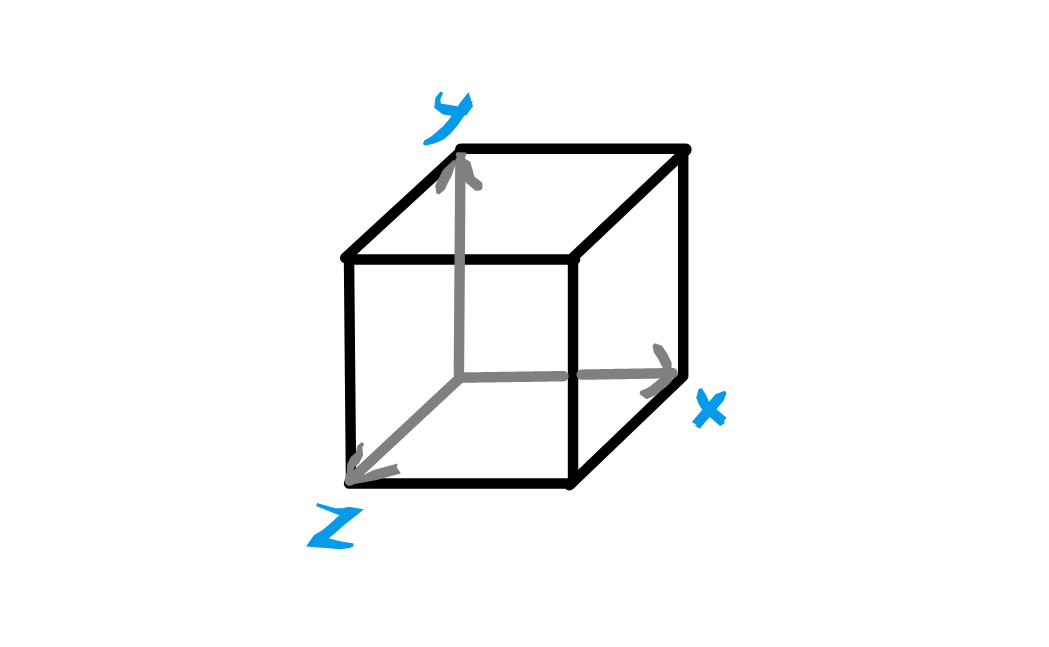
\includegraphics[width=0.86 \linewidth]{local.png}
\end{center}
\end{frame}
\begin{frame}{World space}
    В реальности у нас как правило несколько объектов входящих в 
    сцену. Их расположение относительно друг друга задается в world space 
    системе координат.
\begin{center}
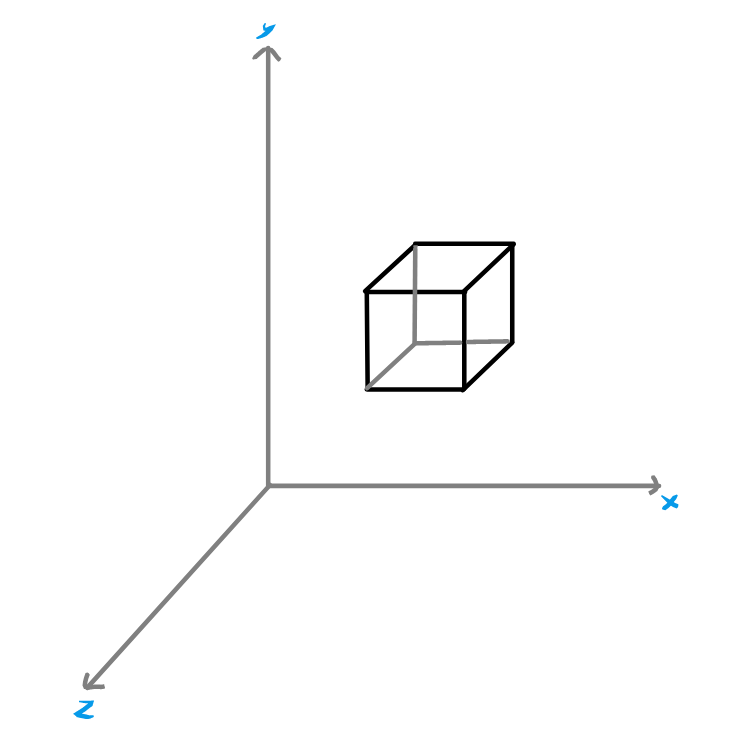
\includegraphics[width=0.5 \linewidth]{world.png}
\end{center}
\end{frame}

\begin{frame}{Преобразования координат}
    Используем 4 координаты для задания точки: $\begin{pmatrix}
        x\\ y\\ z\\ w
    \end{pmatrix}$.

    Это позволяет нам делать аффинные преобразования с помощью матриц.
    Если $w=1$, то можно сделать сдвиг следующим образом:
    \[
        \begin{pmatrix}
            1 & 0 & 0 & \triangle x\\
            0 & 1 & 0 & \triangle y\\
            0 & 0 & 1 & \triangle z\\
            0 & 0 & 0 & 1
        \end{pmatrix}
        \begin{pmatrix}
            x\\ y\\ z\\ 1
        \end{pmatrix} = 
        \begin{pmatrix}
            x + \triangle x\\
            y + \triangle y\\
            z + \triangle z\\
            1
        \end{pmatrix}
    \]
    Помимо сдвигов можно делать обычные линейные операции:
    повороты, растяжения.
\end{frame}


\begin{frame}{View space}
    Хотим получить расположение объектов относительно камеры.

    Это сдвиг + ортогональная замена базиса.
    \[
        M_{view} = \begin{pmatrix}
            r_x & r_y & r_z & 0\\
            u_x & u_y & u_z & 0\\
            -d_x & -d_y & -d_z & 0\\
            0 & 0 & 0 & 1
        \end{pmatrix}\cdot
        \begin{pmatrix}
            1 & 0 & 0 & -p_x\\
            0 & 1 & 0 & -p_y\\
            0 & 0 & 1 & -p_z\\
            0 & 0 & 0 & 1
        \end{pmatrix}
    \]
    $p$ -- позиция камеры

    $r$, $u$, $d$ -- право, верх и направление камеры.

\end{frame}

\begin{frame}{View space}
\begin{center}
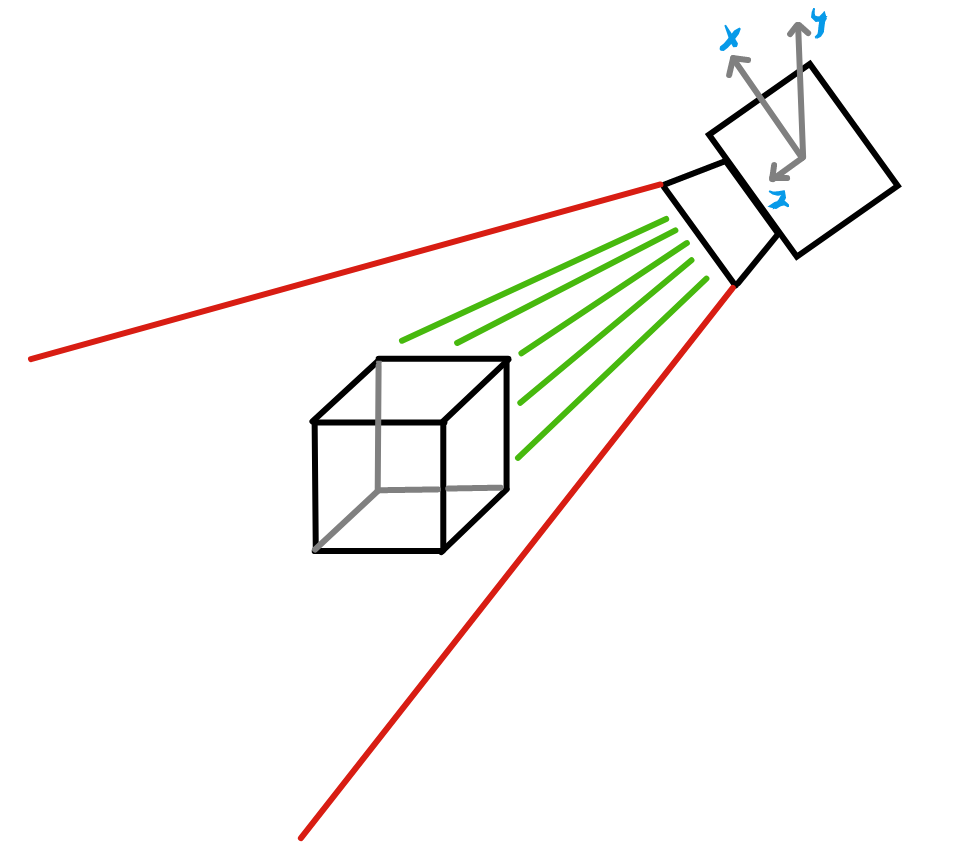
\includegraphics[width=0.7 \linewidth]{view.png}
\end{center}
\end{frame}

\begin{frame}{Clip space}

Перспективная проекция + обрезка(clipping)
\begin{center}
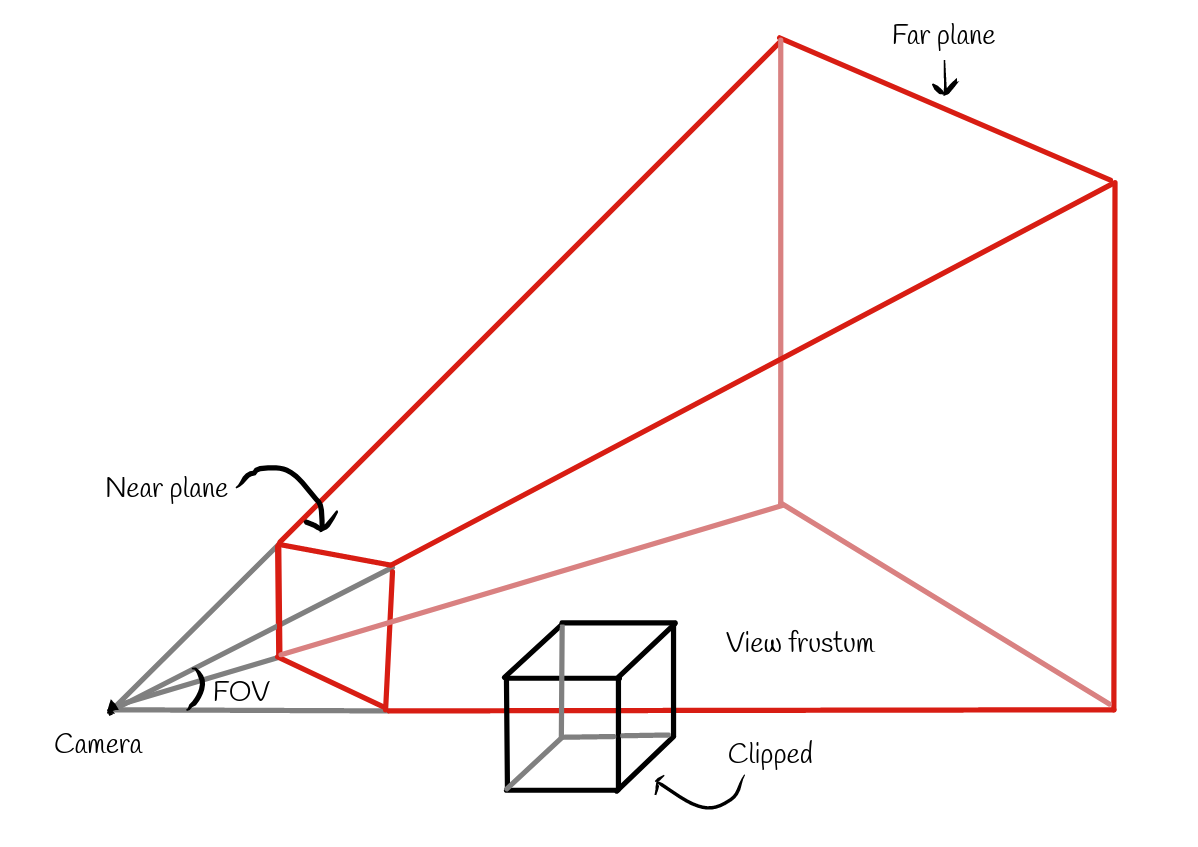
\includegraphics[width=0.8 \linewidth]{my_frustum.png}
\end{center}

\end{frame}

\begin{frame}{Screen space}
    Переходим к пикселям. Целые координаты означают центр 
    пикселя. 
    
    \[
        M_{screen} = 
        \begin{pmatrix}
            w' & 0 & 0 & w'\\
            0 & -h' & 0 & h'\\
            0 & 0 & 1 & 0\\
            0 & 0 & 0 & 1
        \end{pmatrix}
    \]

    $w'$, $h'$ -- половинки ширины и высоты окна.

\begin{center}
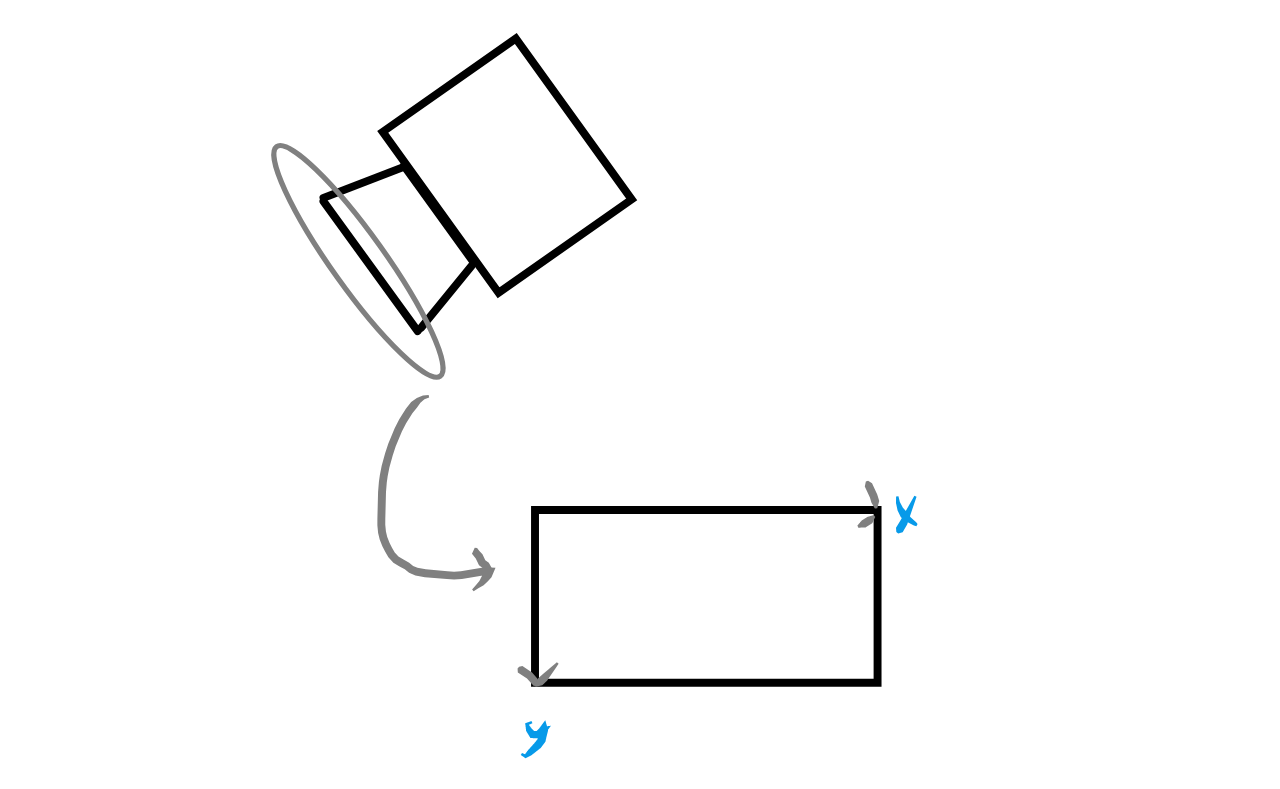
\includegraphics[width=0.6 \linewidth]{screen.png}
\end{center}
\end{frame}

\begin{frame}{Растеризация}
    Хотим понять какие пиксели лежат внутри треугольника и их нужно 
    закрасить, а какие нет.
\begin{center}
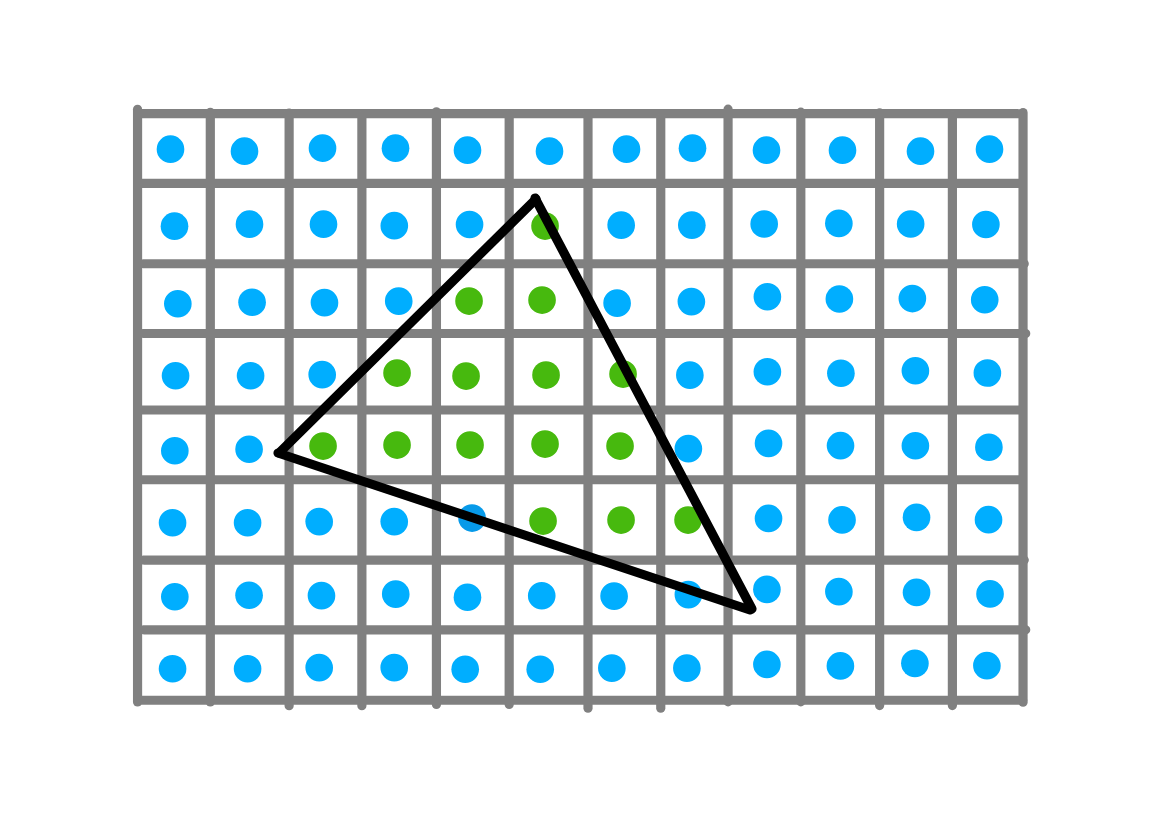
\includegraphics[width=0.8 \linewidth]{rasterization.png}
\end{center}
\end{frame}


\begin{frame}{Растеризация}
%Картинка на которой помечено стрелочками как мы идем
%по long edge, и top edge
\begin{center}
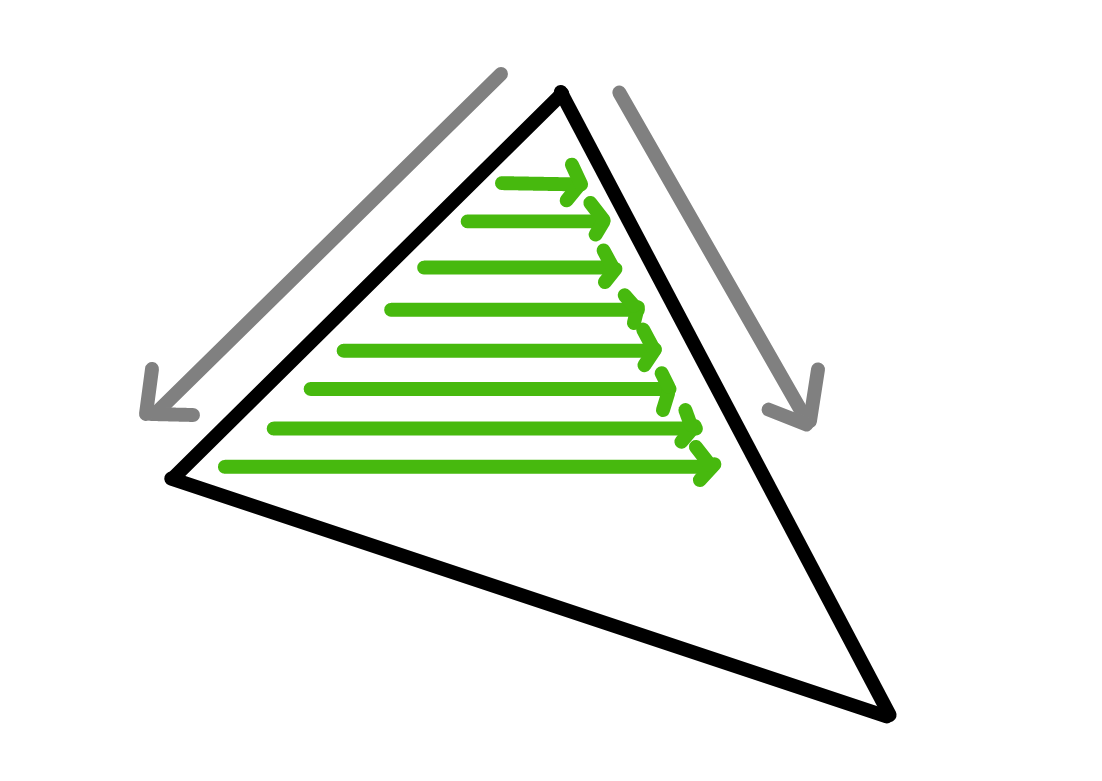
\includegraphics[width=0.8 \linewidth]{algo-1.png}
\end{center}
\end{frame}

\begin{frame}{Растеризация}
%Картинка на которой помечено стрелочками как мы продолжаем
%идти по long edge и идем по bottom edge
\begin{center}
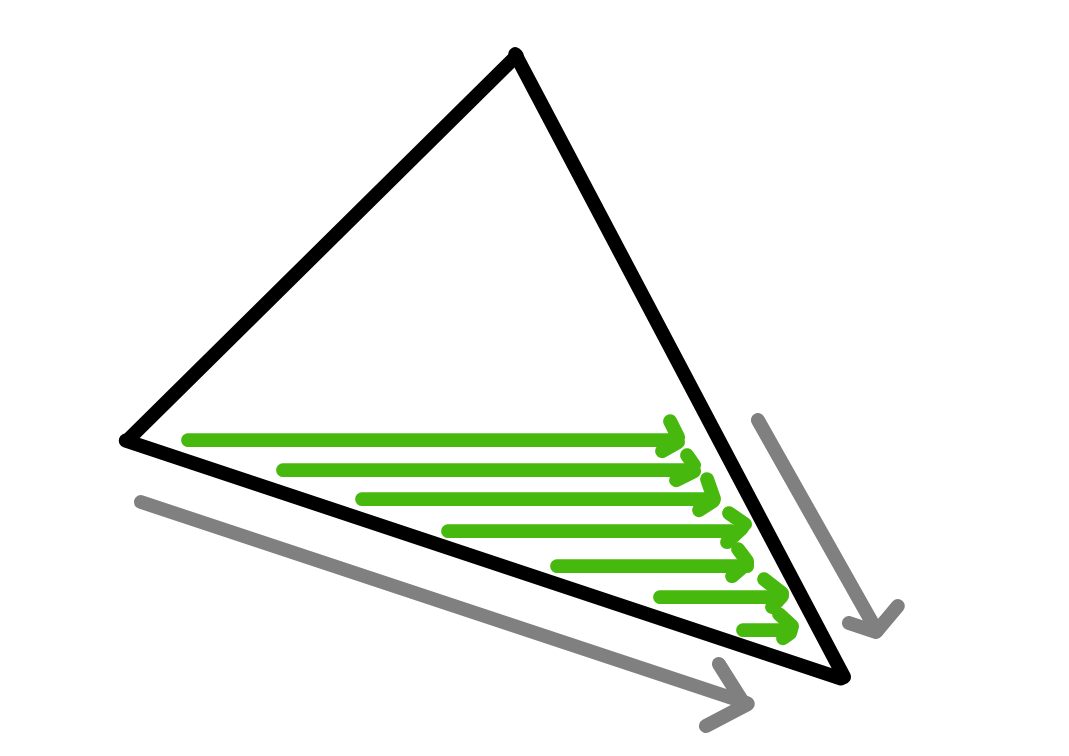
\includegraphics[width=0.8 \linewidth]{algo-2.png}
\end{center}
\end{frame}

\begin{frame}{Буфер глубины}
% TODO: Картиночка?
Сохраняем глубину записанного пикселя в буфер и перезаписываем 
цвет только если глубина уменьшилась. 
\end{frame}

\begin{frame}{Линейная интерполяция}
    Достаточно посчитать градиент линейной функции от координат 
    $x$ и $y$.
\begin{center}
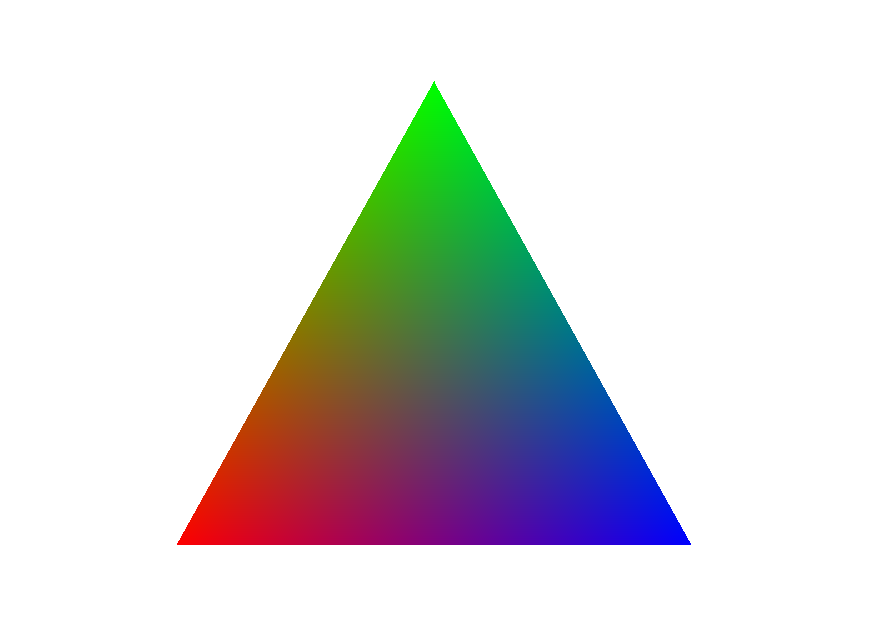
\includegraphics[width=0.8 \linewidth]{gradient.png}
\end{center}
\end{frame}
\begin{frame}{Линейная интерполяция}
    Проблема: зависимость интерполянта от screen space координат 
    не линейная. 

    Решение: для интерполянта $f$ будем интерполировать значение
    $\frac{f}{z}$, а также будем интерполировать $\frac{1}{z}$.

\end{frame}

\begin{frame}{Точечный свет}
В качестве источника света используется точечный свет.
% TODO: Картинка с точечным цветом
\begin{center}

\includegraphics[width=0.8 \linewidth]{lamp.png}
\end{center}
\end{frame}

\begin{frame}{Phong Shading Model}
    Ambient + diffuse + specular
\begin{center}
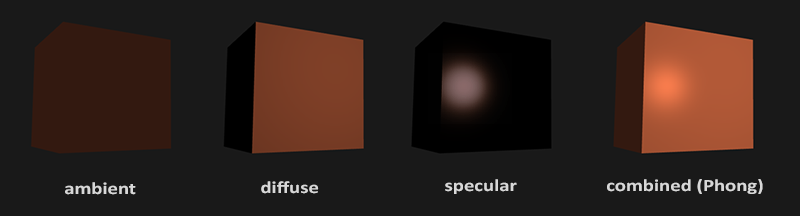
\includegraphics[width=1 \linewidth]{phong.png}
\end{center}
\end{frame}

\begin{frame}{Результаты}
    \begin{center}
    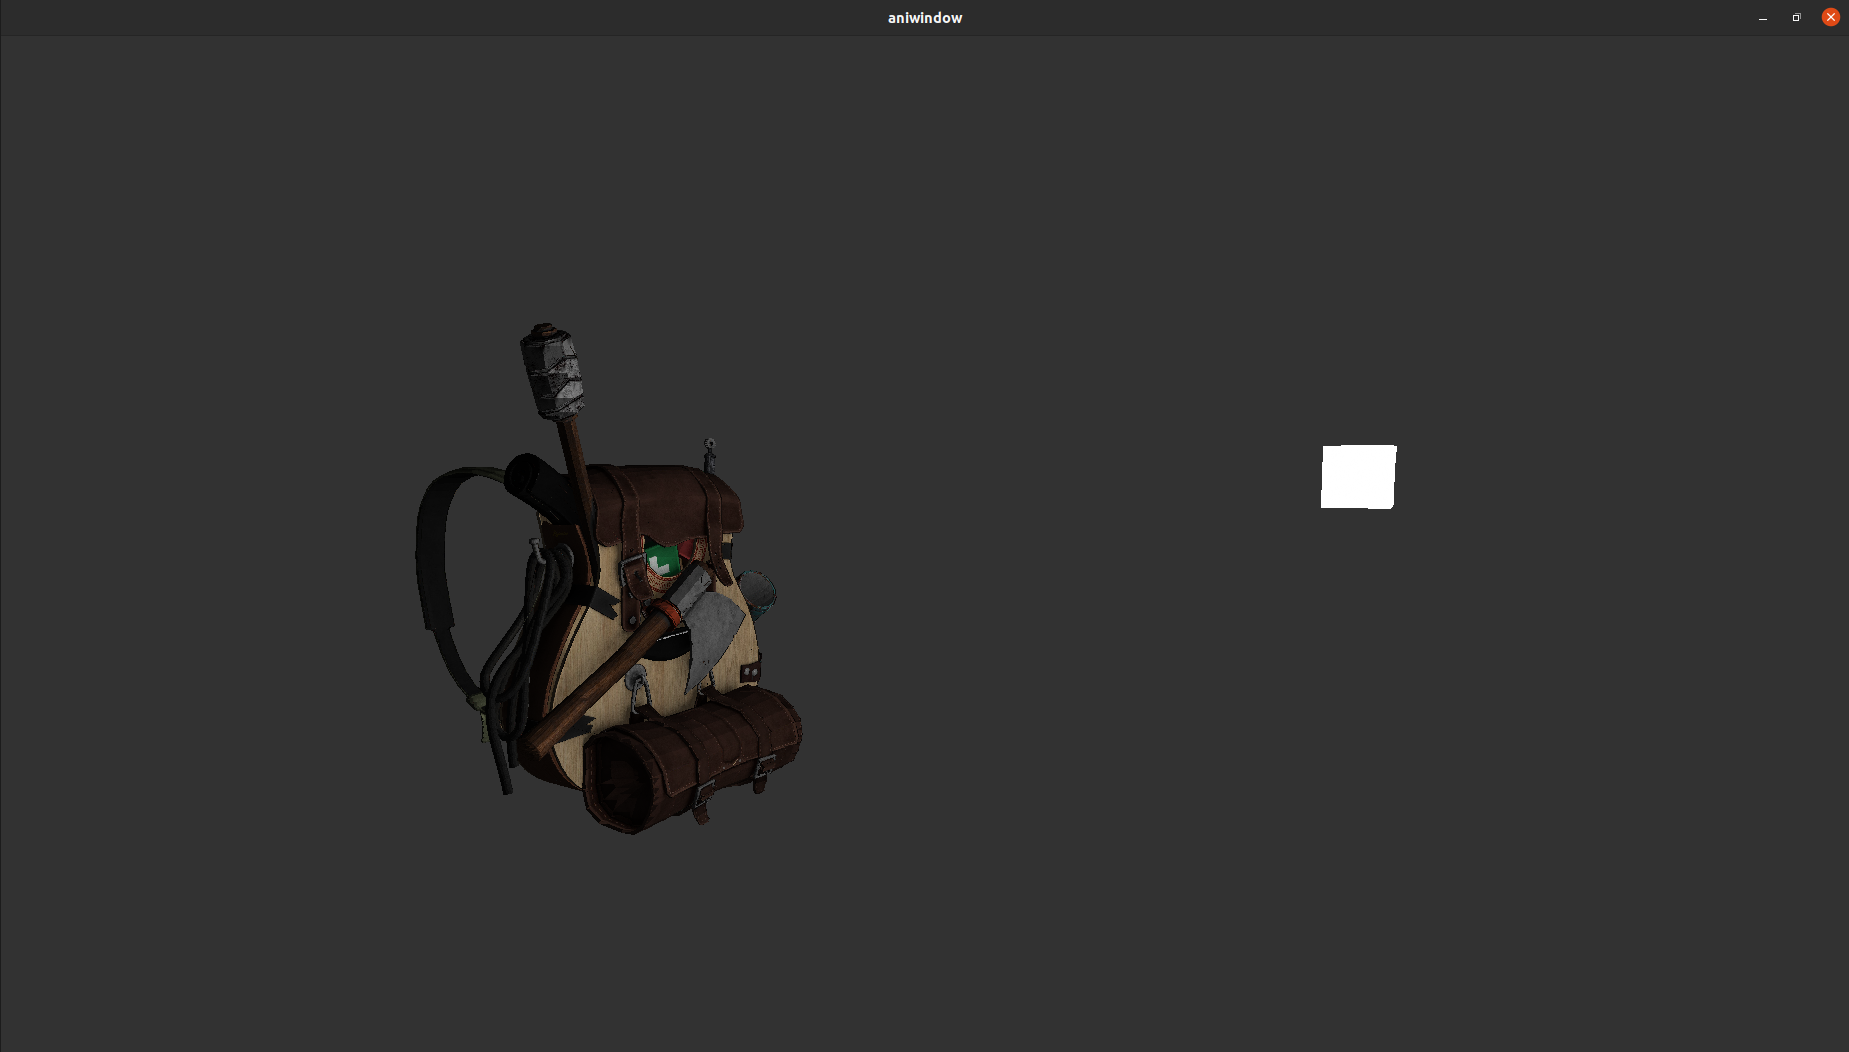
\includegraphics[width=1 \linewidth]{backpack_far.png}
    \end{center}
\end{frame}

\begin{frame}{Результаты}
    \begin{center}
    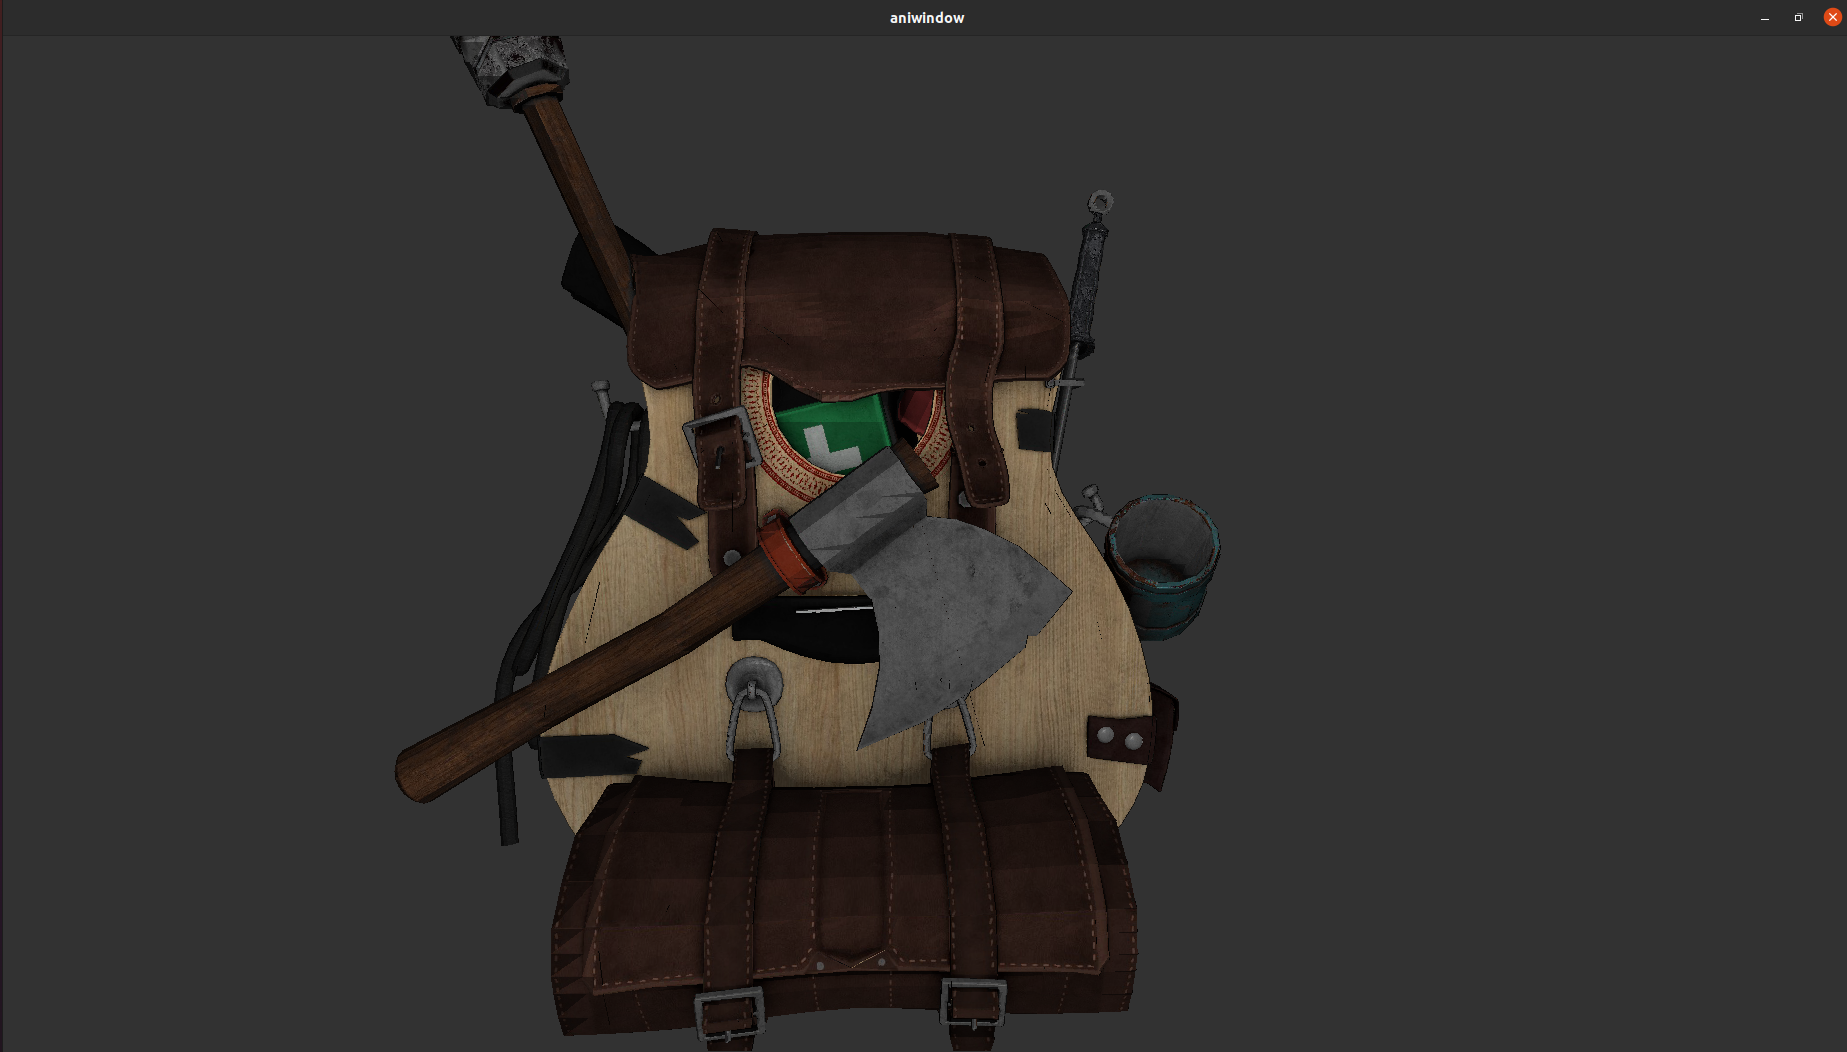
\includegraphics[width=1 \linewidth]{backpack_light.png}
    \end{center}
\end{frame}

\begin{frame}{Результаты}
    \begin{center}
    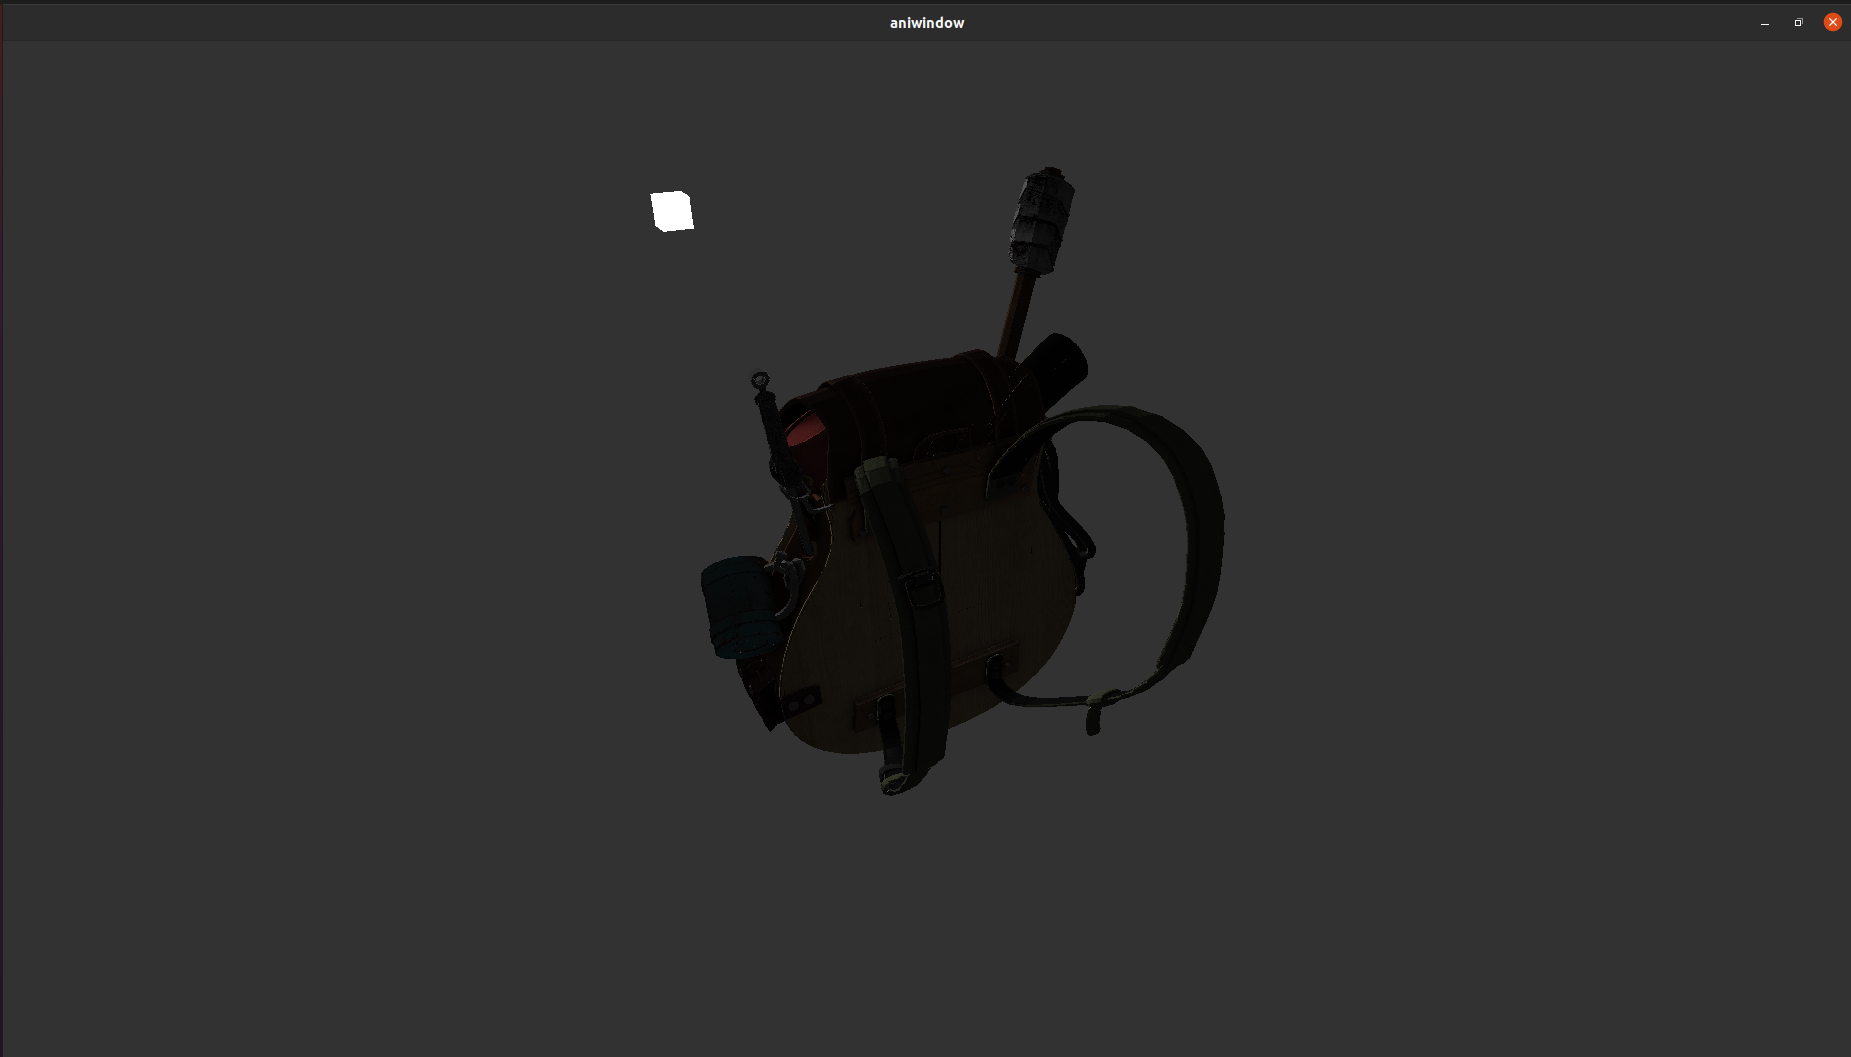
\includegraphics[width=1 \linewidth]{backpack_dark.png}
    \end{center}
\end{frame}

\begin{frame}{Конец}
    \begin{center}
    Спасибо за внимание!
    \end{center}
\end{frame}


\end{document}
